% TEMPLATE for Usenix papers, specifically to meet requirements of
%  USENIX '05
% originally a template for producing IEEE-format articles using LaTeX.
%   written by Matthew Ward, CS Department, Worcester Polytechnic Institute.
% adapted by David Beazley for his excellent SWIG paper in Proceedings,
%   Tcl 96
% turned into a smartass generic template by De Clarke, with thanks to
%   both the above pioneers
% use at your own risk.  Complaints to /dev/null.
% make it two column with no page numbering, default is 10 point

% Munged by Fred Douglis <douglis@research.att.com> 10/97 to separate
% the .sty file from the LaTeX source template, so that people can
% more easily include the .sty file into an existing document.  Also
% changed to more closely follow the style guidelines as represented
% by the Word sample file. 

% Note that since 2010, USENIX does not require endnotes. If you want
% foot of page notes, don't include the endnotes package in the 
% usepackage command, below.

\documentclass[letterpaper,twocolumn,10pt]{article}
\usepackage{usenix,epsfig,endnotes,ctex}
\usepackage{ctex}
\usepackage{graphicx}
\usepackage{multirow}
\usepackage{listings}
\usepackage{array}
\usepackage{fancyhdr}
\usepackage{lastpage}
\usepackage{tikz}

\usetikzlibrary{arrows,shapes,chains}

\begin{document}

%don't want date printed
\date{}

%make title bold and 14 pt font (Latex default is non-bold, 16 pt)
\title{\Large \bf 一种易扩展高可用的分布式订单系统架构}

\author{
{\rm Linqiang Wang}\\
Software Engineer
}

\maketitle

% Use the following at camera-ready time to suppress page numbers.
% Comment it out when you first submit the paper for review.
\thispagestyle{empty}


\subsection*{摘要}
伴随着移动互联网的高速发展、中国第三方支付的快速增长,以及丰富的移动支付产品,深刻改变和培育了中国人民的无现金生活方式,也极大的推进了整个社会经济的发展。对于支付宝和微信支付这样的国民应用,海量交易带来的系统可用性问题成了关乎国计民生的问题。作者有幸参与了微信支付的核心系统的部分开发和改进,也切实感受到支付系统可用性关乎每个产品使用者的产品体验。

本文总结了微信支付的核心订单系统的架构实现,以及海量交易所带来的扩容、成本、容灾和灰度等问题及解决方案,最终通过系统架构多次迭代确立了基于Mysql单机存储引擎,业务和存储强耦的高可用的分布式订单系统。而支付宝走出一条自研高可用分布式存储系统的道路,同样应对了海量的电商交易和双11交易海啸的冲击。本文主要讲述了基于条带构建的高可用分布式订单存储系统,条带是由无状态服务和有状态存储服务组成的条带架构的基本单元,通过条带可以实现线性扩缩容的能力;在下单时通过跳单的操作可以允许一次下单重试更换到可用的条带,这样可以应对少数条带不可用带来的下单不可用问题;同时基于条带的架构也带了冷热分离、故障压缩、差异服务、热点均衡和灰度控制的能力。基于条带化的架构虽然带来很多优点,但同时也造成业务和存储强耦合,另外业务开发人员在开发时也需要了解整体架构不能更加专注业务逻辑。

关键词 - 订单系统、高可用、易扩展、分布式、跳单、条带化、海量存储
\section{简介}
随着移动支付的飞速发展,移动支付用户量持续增加,移动支付已悄无声息的融入到国民的生活并且产生重要的作用。在支付系统中,一笔交易往往需要多个相关系统的协作完成,其中包括支付产品系统、订单交易系统、风控系统、支付系统、账号系统、商户系统、账户系统和清结算系统等等。在一个交易系统中一笔交易是通过一笔订单进行标识的,订单系统需要提供创建订单、支付订单、查询订单、关闭订单和订单退款的能力。订单系统作为其它系统的依赖系统,它的可用性将直接影响整个交易系统的可用性。交易系统的可用性将直接影响用户的交易体验和整个品牌的口碑。

传统的银行都是基于大型的商业服务器和正版授权的数据库软件构建自己的交易系统,互联网有别于传统银行,往往是采用小型廉价的商业服务器和开源的数据库软件构建自己的交易系统。另外传统银行的交易系统是集中式的,而互联网企业多采用分布式系统构建自己的系统,这样对数据的一致性、灾备、可用性提出更高的要求。
对于大型企业或者第三方数据库公司,它们会研发一些自己的分布式数据库存储,例如OceanBase、TiDB等。但是很多企业还是会采用开源的mysql作为自己的数据库系统,一种基于mysql实现的易扩展、高可用支持海量存储的订单交易系统对于是一个企业也是一种很好的方案选择。

本文会讨论一种基于mysql构建的海量订单交易系统,高可用和易扩展作为整个系统两个主要特征。为了达到整个系统的高可用,可用性主要包含三种改进:1)通过使用HaProxy来进行数据库的快速切换解决存储不可用。2)通过条带化进行物理隔离防止单存储故障导致的不可用扩散。3)在系统顶层通过跳单来降低逻辑服务和存储不可用带来的影响。为了解决系统的容量,主要通过条带化单元的水平扩展来扩充整个系统的容量,同时条带化的结构可以很好的解决数据冷热分离的问题。在系统的垂直方向整个系统主要分为代理层、逻辑服务层和存储层;系统在水平方向是由众多物理隔离的条带组成的,一个条带包含了对应的逻辑服务和存储,同时条带也是水平扩展的基本单位。

本文主要先描述整个系统的整体架构,接下来会描述传统架构中存在问题并提出对应的解决方案,然后会讨论整个架构对可用性和易扩展的实现细节,以及探讨结合通用组件来快速开发整个系统。

\section{业界现状}

交易系统的可用性主要分为无状态服务的可用性和有状态存储的可用性,无状态服务的可用性相比更容易解决,而有状态存储服务的可用性则成为整个交易系统的核心瓶颈。为了解决有状态存储服务的可用性,业界也研发了很多的金融级分布式系统存储方案。例如Google的Bigtable、MegaStore和Spanner;Facebook的MyRocks;阿里的OceanBase和X-Engine;腾讯的TDSQL;PingCap的TiDB。这里的存储主要分为两个大的方向:基于关系型数据库构造建分布式关系型存储系统和基于NoSql构建的分布式存储系统。分布式关系型存储系统如OceanBase、MyRocks和TDSQL等;分布式NoSql存储系统如:Spanner、X-Engine和TiDB等。

近代互联网时代,Google的存储技术是整个互联网行业的技术标杆,其发表的GFS、Bigtable和Spanner等一些列技术成果,奠定了近几十年的存储发展方向。其存储系统也经历Bigtable、MegaStore到Spanner的演化,并且Spanner是第一个把数据分布在全球范围内的系统,并且支持外部一致性的分布式事务。不管是在存储的理论研究和技术实现,Google都是这个时代的拓荒者。

Facebook作为一家技术实力同样强劲的互联网厂商, MyRocks是Facebook开发的一款基于RocksDB的开源MySQL存储引擎,并且已经稳定支撑Facebook的海量业务,并作为Facebook的mysql的主分支。

阿里作为中国电商的代表性公司每天都会面临海量的交易,虽然海量交易代表业务的快速增长,但也会对整个交易系统的可用性、扩展性、一致性、性能等提出了更高的要求。在中国移动支付整体快速增长以及阿里的双11活动的推动下,阿里的交易系统也在一次一次的交易海啸中快速成长起来。阿里整个集团不仅完成了去IOE,也完成存储的自研,以及到打磨成为业界顶尖的互联网分布式金融存储产品。阿里目前分布式存储产品有完全自主研发的金融级分布式关系数据库OceanBase和阿里数据库产品事业部自研的OLTP数据库存储引擎X-Engine等。OceanBase作为完全自主研发的金融级分布式关系数据库,支持强一致、高可用、高扩展、高性能、高度兼容和低成本等特性。OceanBase是基于单机关系型数据库,根据数据特性分为基线数据和更新数据构建的一种类Bigtable的分布式存储系统;而X-Engine定位于为阿里云上的公有云客户提供低成本高性能的数据库服务。X-Engine采用了基于LSM Tree的分布式架构,通过优化和借助硬件加速从而提供更低成本下的高性能的读写的OLTP存储解决方案。

伴随着微信支付的快速发展,以及用户持续增长和交易量的增长。腾讯的财付通作为支付底层的服务提供者有自研的金融级分布式数据库TDSQL,不仅支撑微信红包业务,也在腾讯云为更多的企业用户提供分布式数据库解决方案。由于历史原因,微信支付的核心订单系统没有将所有的可用性转移到分布式存储系统,而是走出了一条基于单机关系型数据库,业务和存储强耦的高可用订单系统方案。上面业务和存储强耦的订单存储方案也正是本文讨论的方案,虽然没有采用一些分布式存储方案,但它可能更加适合互联网的中小型企业构建自主的高可用订单存储系统。

除了阿里和腾讯,PingCap是一家专注开源的新型分布式数据库公司,其研发的分布式关系型数据库 TiDB 项目具备分布式强一致性事务、在线弹性水平扩展、故障自恢复的高可用、跨数据中心多活等核心特性,并提供HTAP的一站式解决方案。虽然TiDB没有海量的交易,但作为一家专注存储自研的公司,代表了中国自研存储的努力和崛起。


\section{系统架构}
通过上节的描述,订单交易系统的可用性更加聚焦在有状态存储服务的可用性,一些高可用、强一致的分布式存储方案可以解决问题。也正如前面提到,微信支付的核心订单交易系统没有采用高可用、强一致分布式存储系统,而是走出了一条基于单机存储,存储和业务强耦的一种订单可用方案。这里的方案也可以给更多中小企业提供一种自主构建可用订单系统的解决方案。

\begin{figure}[htbp]
\begin{center}
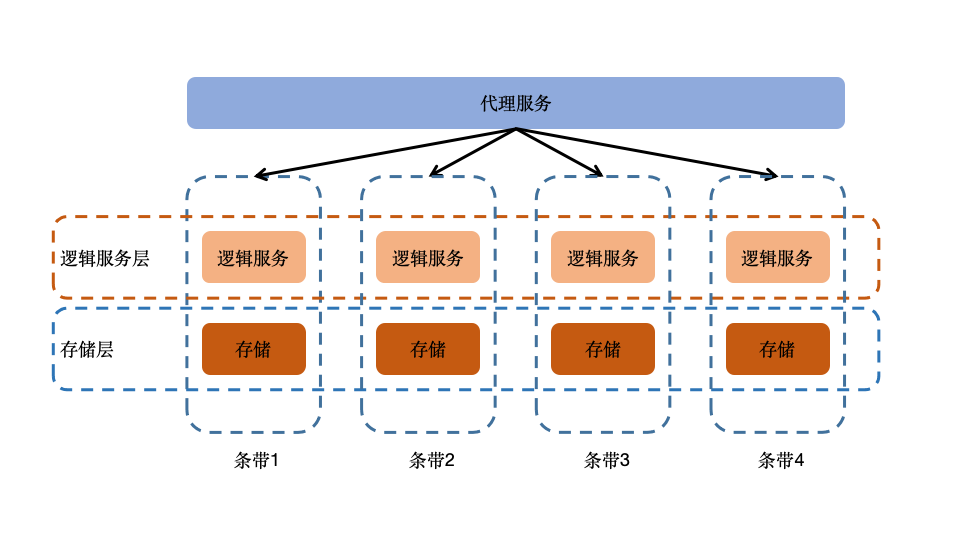
\includegraphics[width=0.5\textwidth]{./figure_1.png}
\caption{订单系统架构概览}
\label{Figure1}
\end{center}
\end{figure}

如图\ref{Figure1}所示的整个系统的简要结构,整个系统是由代理层和若干的条带共同组成的,每个条带内包含无状态的逻辑服务和有状态的存储。整个系统在垂直方向分为三层:代理层、逻辑服务层和存储层。其中,代理层主要功能包含订单路由和跳单、逻辑服务层聚合业务特性、数据的增删改查和单机事务等、存储层负责数据的存储;在水平方向是由多个可动态扩缩的条带组成。

条带是系统构成的基本单元,可以通过条带的逻辑聚合实现读写分离、冷热分离、差异化服务、和提升版本发布质量等。整个系统的容量是通过动态的添加和删除条带来达到容量的动态扩缩容;系统的可用性通过对存储不可用问题提出针对性的解决方案和优化来提升整个系统的可用性。

系统中各条带是物理隔离的,如果存在条单不可用,在代理层可以通过跳过不可用条带保证订单的创建和订单支付有很高的可用性。条单不可用还是会影响该条带内的订单查询和订单退款,实际中订单查询和订单退款相比订单创建和订单支付可以更加柔性和更好的容忍度。通过上面的描述整个系统通过无状态的代理层和跳单共同保证系统的创建订单和支付订单有很高的可用性。条带内的无状态逻辑服务采用三机部署,这样一个条带内所有逻辑服务同时不可用的概率将会极低;条带内的存储也是三机部署,一主两备可以保证集群的数据的灾备和可用性,集群内的主备之间采用半同步保证数据的最终一致(可以采用基于Paxos改造binlog的强一致数据存储,例如PhxSql)。


\subsection{订单号}
基于业务和单机存储强耦的订单存储方案,本质是将存储层的分布式方案上移到业务层进行实现。对于通用分布式存储系统中主键的概念,在分布式订单存储系统中可以天然的使用订单号来代替。存储的分布式一般采用基于Range或者Hash的分片方案,一般先生成好一个全局唯一的主键,然后根据主键决定好数组所在的分片,我们称之为分片先绑定。文章中提出的方案是,通过随机在所有可用的分片中随机选取一个作为当前单号所在的分片,然后将分片的编号记录在到订单号中并进行订单的创建,我们称这种方案为分片迟绑定。

\begin{table}[htp]
\begin{center}
\begin{tabular}{c}
\hline
\hline
\\
订单号 = (版本号,条带编号,时间,订单编号) \\
\\
\hline
\hline
\end{tabular}
\end{center}
\label{default}
\end{table}%

订单号主要由版本号、条带编号、时间信息和订单编号组成。其中版本号用于控制订单号的版本升级;条带编号存储了数据所在的分片,根据条带编号进行路由;时间信息用于记录单号的生成时间,根据时间和访问频率决定数据冷、热和温的程度;订单编号用户保证订单号在全局的唯一性,根据我们的条带方案可以降级到(条带编号,时间信息,订单编号)唯一即可,这样订单编号只需要在一个条带内唯一即可。同时会降低对全局唯一序号生成器的依赖,这样每个条带都可以使用条带内的序号生成器进一步提高整个系统的可用性。

\subsection{路由信息表}
路由信息表维护了每个条带的路由信息,每条路由信息维护了每个条带的编号、逻辑服务的地址和端口、存储服务的地址和端口、条带是否可用、条带的冷、热、温等情况、以及所属分区。
\begin{table*}[htp]
\caption{条带路由信息表}
\begin{center}
\begin{tabular}{|c|c|c|c|c|c|}
\hline
条带编号 & 分区 & 逻辑服务地址 & 存储服务地址 & 可用状态 & 冷热状态 \\
\hline
\hline
0 & 重点商户分区 & Ip:Port  &  Ip:Port  & 可用 & 热 \\
\hline
1 & 普通商户分区 & Ip:Port  &  Ip:Port & 可用 & 热 \\
\hline
2 & 预发布分区 & Ip:Port  &  Ip:Port & 可用 & 热 \\
\hline
3 & 冷分区 & Ip:Port  &  Ip:Port & 可用 & 冷 \\
\hline
4 & 重点商户分区 & Ip:Port  &  Ip:Port  & 可用 & 温 \\
\hline
5 & 普通商户分区 & Ip:Port  &  Ip:Port & 可用 & 温 \\
\hline
6 & 预发布分区 & Ip:Port  &  Ip:Port & 可用 & 温 \\
\hline
7 & 重点商户分区 & Ip:Port  &  Ip:Port  & 不可用 & 热 \\
\hline
... & ... & ... & ... & ... & ... \\
\hline
\end{tabular}
\end{center}
\label{route}
\end{table*}%

如表\ref{route}所示,条带编号是一个增长的ID,没新增一个条带就自增的为条带分配一个新的ID;分区是条带的逻辑聚合概念,我们可以根据聚合的分区构建重点商户分区、普通商户分区、预发布分区和冷分区,从而提供差异服务、冷热隔离等能力。每个条带都有自己的对应的逻辑服务和存储服务,通过配置的地址我们可以在逻辑上形成逻辑隔离的条带,如果机器也不混合部署和重复使用,条带在物理上也是隔离的。可用状态表明当前条带是否可用;冷热状态表明DB中数据的时间特性,我们粗略分为冷、热和温三类。

\subsection{代理服务}
代理服务作为整个订单系统的入口,需要提供下单、支付、查单和关单等接口。下单属于创建订单,支付和关单属于更新订单,查单属于查询订单。下单的时候,代理服务需要正确和均匀的选择条带,并在某些条带不可用的情况下进行跳单保证有限跳单次数内可以找到可用的条带。对于支付、查单和关单需要正确解析单号中的条带信息,进行正确的路由。由于代理服务是无状态的逻辑服务,为了提高代理服务的可用性,通过水平部署多个代理服务实例可以解决。假定同一时刻只有有限个代理服务实例同时不可用,业务方在一次请求中进行失败重试便可将请求路由到其它正常的代理服务,从而保证代理服务具有较高的可用性。

\subsection{条带}
传统的基于Mysql的系统架构中为了扩充系统的容量一般会采用水平的分库分表策略,通过对主键进行哈希将数据分布在不同的机器上从而提升系统的容量。例如实际系统假定有8组DB,可以将主键按8求余进行存储,但是这样的方案存在两个缺点:冷热分离和翻倍扩容。在订单系统中,订单记录在一段时间之后很少会进行订单查询和订单退款,所以具有明显的冷热特性。为了更好的利用机器资源,一般会将x冷数据进行分离并存储到低成本的机器进行存储和访问。对于上面的Sharding模式,我们需要按天建表进行冷数据分离。对于上面的Sharding模式,扩容的时候会选择将DB的数量增加到16组,需要将扩容的数据拷贝一份到新的机器上,然后根据16进行请求重新计算路由,上面的过程被称作翻倍扩容。上面的翻倍扩容对于实时订单系统是无法忍受的,我们更希望对系统的容量进行线性扩缩容,同时不需要影响已经生成的订单。

为了更好的支持冷热数据分离和线性扩容,我们提出基于条带的动态扩容架构。一个条带作为存储的基本单元,其中包含了无状态的逻辑服务和有状态的存储,通过增加和减少条带的数量进行线性的扩缩容。

\subsection{事务}
对于交易系统很多场景下会面临需要操作多个资源同时成功或者失败,如转账、多个单据状态的同时扭转等。在单机关系型数据中我们会使用单机事务来进行解决,同样对于分布式系统需要系统具备分布式事务的能力。由于分布式事务的实现复杂、性能低下等特点,在业务系统中往往会将分布式事务转化为单机事务进行解决,或者将分布式事务根据核心程度划分为主事务和次事务,通过将次事务通过异步组件进行异步补偿完成整个事务。另外,由于交易系统一笔交易往往会操作多个相关的交易单据,我们可以将相关的多个单据部署在同一个分片,这样就可以转化为单机事务进行解决。

通过上面的分析,我们将系统的事务转为条带内的单机事务和跨条带的异常补偿事务,这样各个条带就可以充分解耦做到物理和逻辑的隔离。

\subsection{跳单}
在进行下单前,系统中存在一个条带健康度的检查服务,它会实时模式真实订单探测和收集条带的健康度、耗时等情况。另外,在某些情况下需要手动屏蔽不可用或者可用的条带(如增加或减少跳单,冷热分离等场景)。在下单的时候,代理服务结合条带健康度、黑名单等信息,并在可用的条带内根据短期内每个条带的请求量选择一个可用的条带,然后根据订单号到对应的条带生成订单。
如果第一次成功,则直接返回订单号;如果没有成功,此时可以屏蔽掉当前的条带,进一步在剩余的可用条带内选择一个可用的条带,直到重试到达上限。我们称上面不断重试寻找可用条带的过程为跳单,跳单主要是通过有限次重试跳过不可用条带而保证下单操作的高可用。


\subsection{健康度检查服务}
条带健康度检查服务是所有条带的观察者,它通过周期性模拟真实的交易探测每个条带的可用性和耗时等情况。根据健康度检查服务提供的条带可用和耗时信息可以在下单的时候以更高的概率选到可用的条带而有效的屏蔽掉不可用的条带。条带的是否可用也需要提供好的评价策略和兜底方案,防止网络持续抖动时造成过探测导致所有条带的不可用。

\section{订单流程}
对于订单系统,作为支付系统的核心流程,往往需要提供创建订单、更新订单和查询订单的能力。对于订单的复杂查询,为了不影响实时交易链路的可用性,会采用将备机的数据通过可靠的异步组件同步到非实时的数据库进行复杂查询或者统计等操作。下面会介绍基于上面的条带化架构的创建订单、修改订单和查询订单的流程:

\subsection{创建订单}
如表\ref{create}所示的流程,主要由入口的路由服务完成订单号的生成以及条带不可用时的跳单操作。这样可以保证创建订单的一个高可用,即使存在若干不可用的条带整个系统还是可以进行下单操作。

\subsection{更新订单}
如表\ref{update}所示的流程,当业务在下单流程获取订单号之后,业务方携带单号,代理服务解析单号中的条带编号,就可以保证请求在对应的条带内进行请求,并正确找到对应DB的信息。

\subsection{查询订单}
对于订单查询,我们可以将查询分为实时的读请求和非实时的读请求。实时的读请求读取主库的数据,主要为核心链路提供准确的数据查询;非实时的读请求读取备库的数据,主要为核心链路提供降级的备机读取以及非实时链路的读取。
如表\ref{query}所示的流程,当业务在下单流程获取订单号之后,业务方携带单号,代理服务解析单号中的条带编号,就可以保证请求在对应的条带内进行请求,并正确找到对应DB的信息。


\begin{table*}[htp]
\caption{创建订单流程}
\begin{center}
\begin{tabular}{l}
\hline
\\
1、业务方调用代理服务提供的下单接口进行订单创建。\\
2、代理服务访问跳单健康度检查服务获取当前条带的状态及耗时。 \\
3、根据跳单健康度信息、条带黑名单和条带路由表决定候选的可用条带。\\
4、结合近期每个条带的请求数,然后随机选择一个可用条带作为本次写入的条带。\\
5、调用序列号发生器接口获取全局唯一的订单编号。 \\
6、根据版本号、时间信息、条带编号和订单编号,生成订单号。\\
7、代理服务根据路由信息表在逻辑服务地址中随机选择一个地址,并发出请求。\\
8、逻辑服务根据路由信息表获取存储主机的地址,并建立连接创建订单。\\
9、如果上述过程成功,则返回订单号;否则,跳转到2执行跳单流程,直到成功或者重试次数到达上限。\\
\\
\hline
\end{tabular}
\end{center}
\label{create}
\end{table*}%


\begin{table*}[htp]
\caption{更新订单流程}
\begin{center}
\begin{tabular}{l}
\hline
\\
1、业务方调用代理服务提供的支付、关单或者退款等接口进行订单更新。\\
2、代理服务解析订单号中的条带编号。 \\
3、根据条带编号查询路由信息表获取逻辑服务的地址,并发出请求。 \\
4、逻辑服务根据路由信息表获取存储主机的地址,并建立连接更新订单。\\
5、如果成功;则返回成功;否则返回错误。\\
\\
\hline
\end{tabular}
\end{center}
\label{update}
\end{table*}%

\begin{table*}[htp]
\caption{查询订单流程}
\begin{center}
\begin{tabular}{l}
\hline
\\
1、业务方调用代理服务提供的实时或非实时查询接口进行订单查询。\\
2、代理服务解析订单号中的条带编号。 \\
3、根据条带编号查询路由信息表获取逻辑服务的地址,并发出请求。 \\
4、逻辑服务根据路由信息表获取存储主机的地址,并建立连接查询订单。\\
5、如果成功;则返回成功;否则返回错误。\\
\\
\hline
\end{tabular}
\end{center}
\label{query}
\end{table*}%

\section {架构特性}
\subsection {线性扩容}
对于海量交易的系统,线性扩容成为一个重要的特性。线性扩容给整个系统提供了更多的灵活性以应对特定时期的交易洪峰,并且能通过简单的扩缩容取得交易处理能力和成本的平衡。对于业务可能快速持续增长的系统,线性扩容能力可以应对不必要的系统重新设计和重构。

\subsection {故障压缩}
由于各条带是逻辑和物理隔离的,不管是由于条带内DB导致的故障或者灰度发布导致的故障,相应的故障只会压缩在该条带内,不会扩散导致整个系统的雪崩。通过统计我们可以简单估算每个条单不可用的概率,然后估算整个系统不可用的概率。

\subsection {差异服务}
根据我们抽象的条带概念,我们可以再聚合某些条带为一个分区,某些商户的请求只可以落在某些分区的条带内。这样不同的分区提供不同的机器、带宽等,可以实现对重点商户和非重点商户的差异化服务。

\subsection {冷热分离}
当系统某些条带的容量到达预警值,或者其中的数据已经超过某个冷却阈值。我们可以将条带变为只读和可更新,但不能再进行数据的写入。等到数据的访问量下降到某个阈值后,可以将条带内的全量数据停写后拷贝到冷库,然后修改条带路由信息中的存储服务地址为冷数据所在的新机器的地址。然后删除旧机器上的数据并新增一个空的条带,这样就可以简单的完成冷热数据分离,同时上面的过程可以实现完全自动化。

\subsection {灰度控制}
在互联网系统的可用性问题中,统计发现很多版本的问题可以通过合理的灰度提早发现和解决。基于条带的架构可以轻松的构建预发布环境,预发布环境通过后可以控制新版本先对某些生产条带进行灰度发布,然后逐步灰度到所有的条带。同时还可以通过控制某些条带的请求量从而可以做到更细粒度的灰度。

\subsection{热点均衡}
在选择分区的时候,可以统计近期每个条带创建的订单数作出一个合理的条带选择,从而达到最大程度的数据均衡,避免传统分片模式下数据倾斜的问题。

\section{备份、容灾和恢复}

\subsection{备份}
为了应对机架级不可用、机房级不可用和城市级不可用,需要通过数据备份进行容灾。可以根据业务的容灾选择合理的容灾级别,通常业务会选择一主两备的三机备份策略。

\subsection{数据一致性}
如果采用Mysql作为条带内的存储引擎,Mysql支持同步复制、异步复制、半同步复制、增强半同步复制和MGR(MySQL Group Replication)。通常我们很少采用同步和异步复制,在Mysql5.7增强半同步之前DBA多会采用半同步复制,但如果主机宕机切换到备机会出现一定的数据不一致。为了解决半同步带来的问题,Mysql5.7之后推出了增强半同步。但是MGR是基于Paxos的强一致复制方案,但是MGR业界的互联网公司却很少有公司采用。

\subsection {容灾}
我们假定所有的机房都在一个城市内的不同机房,为了应对城市内的机房级不可用,我们需要将三份数据分布在同城的三个不同机房内,同时保证每个机房内有相同的主机和备机的数量,对机房级进行负载均衡。当出现机房级以及机房级以下的不可用,可以快速的进行主机切换保证业务的可用性,如果出现整个机房的不可用最多会损失1/3的交易量。但是对于条带化的架构,我们可以快速调整条带路由信息表将不可用的条带进行屏蔽,这样只会有一个短暂的不可用。

\section{架构缺点及改进}
\begin{itemize}
\item 1、对于分布式事务不太友好。
\item 2、其实可以将更多的能力下降到存储进行解决,这样对业务人员的架构能力提出较高的要求。
\item 3、如果现行系统进行改造的成本过高。
\end{itemize}

\section{总结}

上文首先描述了基于单机Mysql构建的业务和存储强耦合的高可用海量分布式订单系统,基于抽象的条带概念使得整个系统架构天然具备了一些线性扩容、故障压缩、冷热分离、灰度控制、差异服务和热点均衡等能力。虽然不同于支付宝通过强一致分布式存储系统来保证分布式存储服务的高可用,但这种构建于单机Mysql的架构更加适合没有独立研发分布式存储的中小企业。从目前业界存储演进的方向来看,强一致的分布式关系型数据存储系统还是业界努力的方向。

\end{document}







